%% 美赛模板:正文部分

\documentclass[12pt]{article}  % 官方要求字号不小于 12 号,此处选择 12 号字体
% 本模板不需要填写年份,以当前电脑时间自动生成
% 请在以下的方括号中填写队伍控制号
\usepackage[MI00008]{easymcm}  % 载入 EasyMCM 模板文件
\problem{B}  % 请在此处填写题号
 \usepackage{mathptmx}  % 这是 Times 字体,中规中矩 
%\usepackage{mathpazo}  % 这是 COMAP 官方杂志采用的更好看的 Palatino 字体,可替代以上的 mathptmx 宏包
\title{An MCM Paper Made by Team MI00008}  % 标题
\usepackage{enumerate}
% 如需要修改题头(默认为 MCM/ICM),请使用以下命令(此处修改为 MCM)
%\renewcommand{\contest}{MCM}
\usepackage{bm}
\usepackage{cleveref}
% 文档开始
\begin{document}

% 此处填写摘要内容
\begin{abstract}
    Here is the abstract of your paper.
    Firstly, that is ...

    Secondly, that is ...

    Finally, that is ...

    % 美赛论文中无需注明关键字。若您一定要使用,
    % 请将以下两行的注释号 '%' 去除,以使其生效
    \vspace{5pt}
    \textbf{Keywords}: MATLAB, mathematics, LaTeX.

\end{abstract}

\maketitle  % 生成 Summary Sheet
\tableofcontents  % 生成目录


% 正文开始
\section{Introduction}
\subsection{Problem Background}
China has been undergoing a period of political, economic, social, and cultural system transformation since the reform and opening up. At the same time that urbanization has accelerated and various new and old types of contradictions and conflicts have persisted, the functioning of the social system has been disrupted, which has forced society to transform in an unbalanced and uncoordinated way. The complexity and unpredictability of society have substantially expanded in the age of worldwide informationization, along with the rapid growth of the economy, and risk factors have multiplied around people's everyday lives, altering how they perceive social security and stability. 

The brutal terrorist attack in Kunming, the explosion accident in Tianjin Binhai New Area, the Changchun Changsheng vaccine incident, and the repeated outlawing of environmental pollution and economic aid crimes all strongly suggest the emergence of a risk society. As a result, China must now grapple with the issue of how to preserve social harmony and stability while the country is developing economically and socially and reduce the negative effects of multiple risk events.
\subsection{Problem Restatement}
\begin{itemize}
\item \textbf{For problem 1:} We are required to select representative indicators in various aspects to reflect various aspects of social stability. And from a qualitative and quantitative point of view, establish a system of indicators of social stability, and discuss their interrelationship.
\item \textbf{For problem 2:} We need to establish an early warning model for social stability based on the indicator system that affects social stability established in the first question, and discuss it.
\item \textbf{For problem 3:} We need to select a country or region that has had a color revolution and use the indicator system and early warning model established by our first and second questions to assess its social stability. And find out the main reasons or factors for the failure of this color revolution, judge the trend of future social stability, and put forward our suggestions.
\item \textbf{For problem 4:} Find a country where color revolutions have led to regime change, and use the model we have built to find the main causes of regime change.
\item \textbf{For problem 5:} Put forward our team on the prevention of color revolution, maintain social stability recommendations.
\end{itemize}
\subsection{Our work}
Previous research in this area has been very in-depth, and domestic research on the social stability index system is endless. Only then can we use its research results to solve the problems we encounter. Here's our work:

Based on the theory of risk society and social governance, this paper summarizes the relevant literature of social stability and its measurement, and discusses the construction of social stability index and index system. 

Based on the research and analysis of social stability risk sources, a dimensional model of social stability index was constructed. Then, according to the principles of data availability, scientificity, and operability, specific indicators are set and selected, and a complete index system framework is gradually built to analyze the actual operation and results of the social stability index.

Based on the determination of various indicators and weight distribution models of the social stability index, the research objects that have occurred in the color revolution were selected to evaluate their social stability, and the main risk factors affecting social stability in the color revolution were identified.
\begin{figure}[htbp]
\centering
\begin{subfigure}[b]{\textwidth}
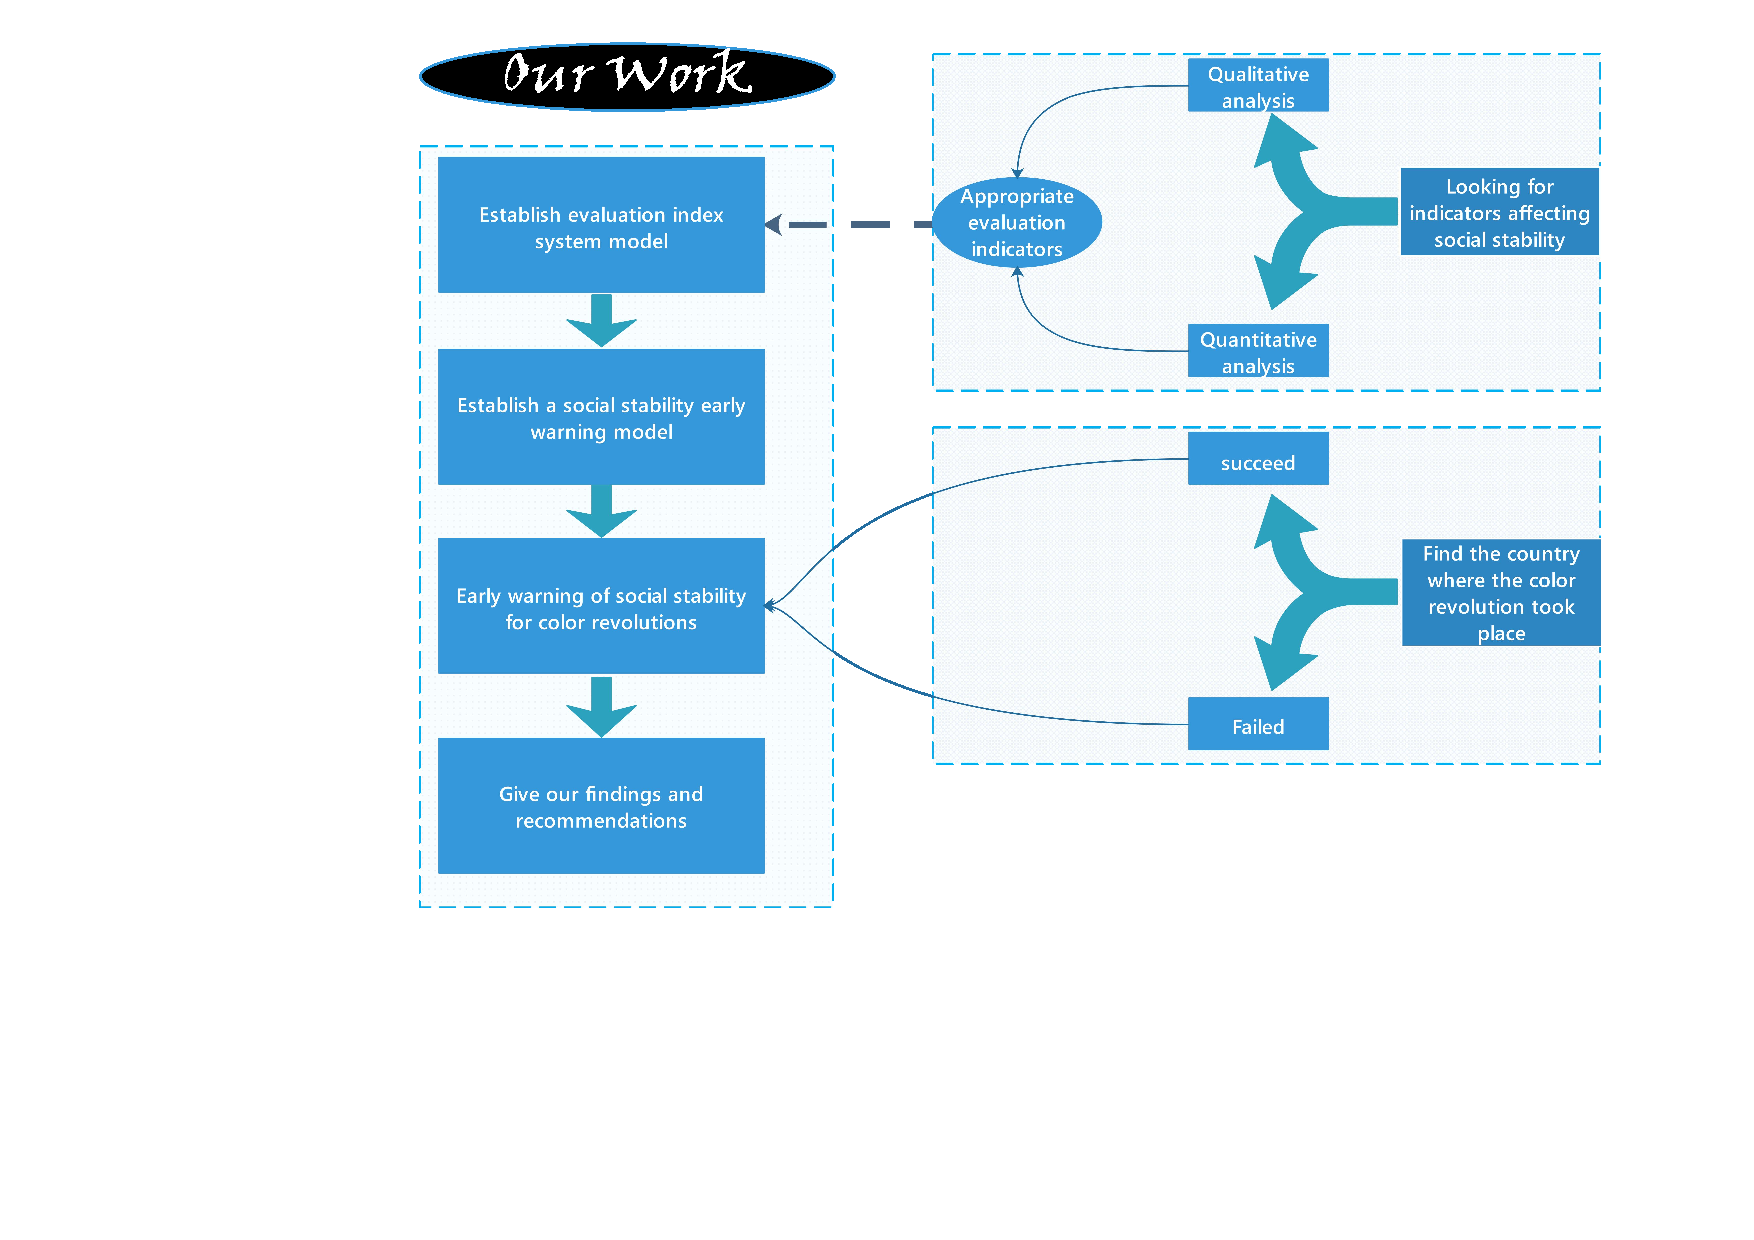
\includegraphics[width=\textwidth]{img/our work.pdf}
\end{subfigure}
\end{figure}
\section{Preparation of the Models}
\subsection{Assumptions}

\subsection{Notations}
The primary notations used in this paper are listed in Table \ref{tb:notation}.

% 三线表示例
\begin{table}[!htbp]
\begin{center}
\caption{Notations}
\begin{tabular}{cc}
	\toprule
	\multicolumn{1}{m{3cm}}{\centering Symbol}
	&\multicolumn{1}{m{8cm}}{\centering Definition}\\
	\midrule
	$A_i$&Level 1 indicators\\
	$A_{ij}$&Level 2 indicators\\
	$A_{ijk}$ &Level 3 indicators\\
	$SRD$&Social Risk Degree\\
	\bottomrule
\end{tabular}\label{tb:notation}
\end{center}
\end{table}













\section{Establishment of Our Model}
\subsection{Unascertained Measure Model}
Let $r_1,r_2,\cdots ,r_m$ be $m$ objects to be optimized, then $\bm{R}=\{r_1,r_2,\cdots ,r_m\}$ can represent the space to which the object to be optimized belongs.
Each $r_i(i = 1,2,\cdots ,m)$ consists of $n$ evaluation indexes. Recorded as $t_1, t_2,\cdots ,t_n$. 
Use $\bm{T}=t_1, t_2,\cdots ,t_n$ to represent the evaluation index space of $r_i$ ,then $r_i$ can be expressed as an n-dimensional vector $\bm{r_i}=\{r_{i1},r_{i2},\cdots ,r_{in}\}$. 
The observed value of the evaluation index is expressed by $r_{ij}(i=1,2,\cdots , m; j=1,2,\cdots ,n)$. 
Suppose that each $R_{ij}$ has $p$ evaluation levels, denoted $C_1,C_2,\cdots ,C_p$. 
Then the overall evaluation space can be denoted as $\bm{C}={c_1,c_2,\cdots ,c_p}$. 
Among them, the $k$ evaluation grade can be expressed by $c_k(k=1,2,\cdots ,p)$, and if the $k$ level is greater than the $k+1$ level, it is written as $c_k>c_{k+1}$.
If there is $c_1>c_2>\cdots >c_p$ or $c_1<c_2<\cdots <c_P$, then $c_1, c_2,\cdots ,c_p$ is an ordered division class.
\begin{enumerate}
    \renewcommand{\labelenumi}{\textbf{Step \theenumi}}
    \item Measurements $r_{ij}$ of the $k$ rating level $c_k$. The degree is expressed asin the $u_{ijk}=u(r_{ij}\in c_i)$, requirement $u$ to meet:
\begin{eqnarray}
    &0\le u(r_{ij}\in c_k)\le 1
    \label{e1}\\
    &u(r_{ij}\in C)=1
    \label{e2}\\
    &u(r_{ij}\in U_{i=1}^kc_i)=\sum_{i=1}^{k}u(r_{ij}\in c_i)\label{e3}
\end{eqnarray}
Thereinto, $i=1,2,\cdots ,m$

\hspace{4.5em}$j=1,2,\cdots ,n$

\hspace{4.5em}$k=1,2,\cdots ,p$.\\
Thereinto, Equation \ref{e1} represents ``non-negative boundedness'', Equation \ref{e2} represents ``normalization'', Equation \ref{e3} represents ``additivity''. The $u$ that simultaneously satisfies the Equation \ref{e1} to Equation \ref{e3} is called an unascertained measure, and has a single index measure matrix $(u_{ijk})_{n\times p}$:
\begin{equation}
    (u_{ijk})_{n\times p}=\begin{bmatrix}
  u_{i11}&u_{i12}  &\cdots  &u_{i1p} \\
 u_{i21} &u_{122}  &\cdots  &u_{i2p} \\
\vdots  & \vdots   & \ddots &\vdots  \\
  u_{in1}&u_{in2}  &\cdots  &u_{inp}
\end{bmatrix}
\end{equation}
\item According to the grading standard of the evaluation index and the measured value of each index, the comprehensive measurement evaluation matrix of the index is determined, and the comprehensive measure of multiple indicators is calculated in combination with the comprehensive index weight determined by the improved entropy weight method, which is as follows (Wang Xinmin et al., 2012):
\begin{equation}
    u_{ik}=\sum_{j=1}^{n}w_ju_{ijk}
\end{equation}
Thereinto, $i=1,2,\cdots ,m$

\hspace{4.5em}$j=1,2,\cdots ,n$

\hspace{4.5em}$k=1,2,\cdots ,p$.
\item Calculate $u$ as:
\begin{eqnarray}
    &0\le u_{ik}\le 1\\
    &u(r_i\in C)=\sum_{k=1}^{p}u_{ik}=1\\
    &u(r_i\in \bigcup_{l=1}^{k}c_l)=\sum_{l=1}^{k}u(r_i\in c_l)
\end{eqnarray}
Therefore, the object of evaluation is obtainedriThe p-dimensional vector of the multi-index comprehensive measure of , which can be expressed as $\bm{U}=\{u_{i1},u_{i2},\cdots ,u_{ip}\}$. 
\item Multi-indicator evaluation matrix $(u_{ik})_{m\times p}$ as follows:
\begin{equation}
    (u_{ik})_{m\times p}=\begin{bmatrix}
 u_{11} &u_{12}  &\cdots   &u_{1p} \\
  u_{21}&u_{22}  & \cdots  &u_{2p} \\
  \vdots & \vdots &  \ddots & \vdots\\
 u_{m1} &u_{m2}  &\cdots   &u_{mp}
\end{bmatrix} 
\end{equation}
    \item In order to determine the weight of each indicator, the evaluation level of the gold cave tailings pond was calculated by using the confidence identification criterion. Set the reliability to $\lambda$ and $\lambda \ge 0.5$. If $c_1>c_2>\cdots >c_p$, its recognition model is:
    \begin{equation}
        \min \{k:\sum_{l=1}^{k}u_{il}\ge \lambda,1\le k\le p\}
    \end{equation}
Thereinto,$k=1,2,\cdots ,p$,$s$ is the degree of affiliation. When the value of $k$ satisfies the recognition model, the membership degree $s$ is calculated to obtain the evaluation objectriBelongs to the $s$ rating and is credited as $c_s$.
    \item After deriving the security level of the evaluated object according to the confidence identification criterion, it is also necessary to rank the degree of influence of the influencing factors. If the ordered evaluation space is $\{c_i\}$, then $c_k$ of the value equals to $e_k$, and $e_k>e_{k+1}$. Then we have:
    \begin{equation}
        q_{Bi}=\sum_{k=1}^{p}e_ku_{ik}
    \end{equation}
Thereinto,$q_{Bi}$ is the importance of the unascertained measure, and the importance vector of the unascertained measure $q=\{q_{B1}, q_{B2},\cdots , q_{Bn}\}$. The influence degree of the influencing factors is ranked by comparing the size of $\rm{q}$.
\end{enumerate}
\subsection{ISM Model}
ISM (Interpretive Structural Modeling) is a model that is developed to study complex systems. 
Based on tools such as directed graph, matrix and computer technology, a multi-level 
hierarchical structure model is constructed (POLAT \& RMAC, 2011, p. 169-174). DEMATEL 
(Decision Making Trial and Evaluation Lab), which is a scientific method based on graph theory 
and matrix to simplify the complex system structure (Gu Xuesong \& Chi Guotai, 2010, p. 508-
514). The combined model in this paper integrates the centrality and causation of DEMATEL 
into the multi-level hierarchical structure of ISM, which can not only clarify the hierarchical 
relationship of various influencing factors but also study the relative importance of constraints, 
so as to make the analysis result more objective and reasonable.
The steps to build the composite model are as follows:
\begin{enumerate}
    \renewcommand{\labelenumi}{\textbf{Step \theenumi}}
    \item Determine the set of influencing factors :
\begin{equation}
A=\{a_i|i=1,2,\cdots ,n\}
\end{equation}
    \item Determine the factor influence scale, and determine the mutual influence relationship between 
the factors through expert knowledge and experience, and get the direct influence matrix $V$.
\begin{equation}
    V=[v_{ij}]_{n\times n}
\end{equation}
Thereinto, $v_{ij}$ represents the influence degree of factor $a_i$ on factor $a_j$. When $i=j$ , $v_{ij}=0$.
    \item  Calculate the direct impact matrix $V$ to obtain the normalized direct impact matrix $X$ :
    \begin{equation}
X=[X_{ij}]_{n\times n}=\frac{V}{\max \sum_{j=1}^{n}V_{ij}}
\end{equation}
    \item Calculate the comprehensive impact matrix $T$ :
\begin{equation}
T=[T_{ij}]_{n\times n}=X(I-X)^{-1}
\end{equation}
Thereinto, $I$ is identity matrix.
    \item The influence degree $f_i$ , the influence degree $e_i$ , the center degree $z_i$ and the reason degree $y_i$ of 
the constraint factors were calculated. The calculation formula is as follows:
\begin{eqnarray}
    &f_i=\sum_{j=1}^{n}T_{ij},1\le i\le n \\
    &e_i=\sum_{j=1}^{n}T_{ij},1\le i\le n\\ 
    &z_i=f_i+e_i\\
    &y_i=f_i-e_i
\end{eqnarray}
    \item Draw the cause and result diagram:

Cartesian coordinate system is drawn with the degree of center as the abscissa and the degree of 
cause as the ordinate.
    \item  Calculate the overall impact matrix $H$ :
    \begin{equation}
        H=[H_{ij}]_{n\times n}=T+I
    \end{equation}
    \item Determine the threshold value $\lambda$ (Xue Wei1 \& Geng Zhiwei, et al. 2019, p. 99-104.):
\begin{equation}
    \lambda =\alpha +\beta
\end{equation}
Where, and respectively refer to the mean value and standard deviation of the comprehensive 
influence matrix $T$ .Different $\lambda$ values have different logical relationships with the 
influencing factors (Sun Jing, 2018). The choice of $\lambda$ is more subjective based on expert 
experience, while replacing it with the sum of the mean and standard deviation based on the 
statistical distribution is more objective, which can reduce the influence of subjectivity.
    \item Calculate the standardized reachable matrix $K$ :
\begin{equation}
    K=[K_{ij}]_{n\times n}
\end{equation}
Thereinto, if $H_{ij}>\lambda$ ,then $H_{ij}=1$ 

\hspace{4.5em} if $H_{ij}\le \lambda$ ,then $H_{ij}=0$ .
\item  According to the reachability matrix, the reachability set $R_i$ and antecedent set $S_i$ of each 
influencing factor are determined.\\ 
Thereinto, $R_i$ is composed of the index set corresponding to all the 
columns with index 1 in the ith row of the reachable matrix

\hspace{4.5em} $S_i$ consists of the set of indices 
corresponding to all rows with index 1 in the ith column of the reachable matrix.
\item Verify:
\begin{equation}
    R_i=R_i\cap S_i,(i=1,2,\cdots ,n)
\end{equation}
If it is true, then $a_i$ is the highest level factor. At this time, row $i$ and column $i$ are deleted in $K$ , 
and the calculation is repeated until all factors are deleted.
\item Draw the hierarchical structure diagram of factors according to the order of factors to be 
deleted, and establish the structural model.
\end{enumerate}
\subsection{DEMATEL Model}
The decision experiment and evaluation laboratory method, or DEMATEL, is a mathematical language for quantifying complex system problems by using graph theory and matrix tools. DEMATEL obtains the degree of centrality and the degree of cause by calculating the degree of influence and the degree of being affected, and then analyzes the dependence among the factors. The steps for the DEMATEL method are as follows.
\begin{enumerate}
    \renewcommand{\labelenumi}{\textbf{Step \theenumi}}
\item The object factors are determined, and the direct influence matrix $X$ is established according to the logical relations among the factors.

\item Matrix normalization process, sum the rows of matrix $X$, set its value to $Sum_i (i=1,2,\cdots ,n)$, find the maximum value $Sum_{max}$, let $X'=X/Sum_{max}$, get the normalized matrix $X'$.
\item Calculating the comprehensive influence matrix $T$, calculating the matrix $T$ according to the formula $T = X'(I-X')^{-1}$, where $I$ is the unit matrix.
\item The influence degree ($T$), the affected degree ($R$), the center degree ($P$) and the reason degree ($E$) were calculated according to the comprehensive influence matrix $T$.
\item Dawing the distribution map of the influencing factors according to the centrality and the degree of cause.
\item The causal factor group and the result factor group were analyzed iteratively, and the causal hierarchy diagram was drawn.
\end{enumerate}
\subsection{Establishment of DEMATEL-ISM Model}
DEMATEL-ISM was proposed by American scholars. By combining adjacency matrix and direct influence matrix, this method decomposes the complex system into multi-level hierarchical form with clear hierarchy, quantifies the risk factors, studies the influence degree and affected degree of risk factors, and obtains the hierarchical structure relationship of risk factors.

DEMATEL-ISM combines DEMATEL and ISM theories, which can effectively determine the causal relationship between factors, obtain the hierarchical structure of influencing factors, excavate the deep-seated factors leading to accidents, and thus provide a theoretical basis for the proposal of accident prevention measures.

In order to fully analyze the influencing factors of social stability, the DEMATEL-ISM method is specially used to analyze the key factors and core factors that cause accidents, providing theoretical support for preventing accidents. The specific process is as follows: build the impact matrix, determine the impact strength between the factors affecting the fire and explosion accidents in the laboratory, determine the direct impact matrix and normalize it. 
\begin{enumerate}
    \renewcommand{\labelenumi}{\textbf{Step \theenumi}}
\item According to Unascertained Measure Model and ISM Model, the intensity of action between the influencing factors was analyzed, and the values were assigned according to 5 levels, including no influence 0, small impact 1, average impact 2, large impact 3 and severe impact 4, and two initial direct impact matrices were obtained. To eliminate the fluctuation between fractions, the 2 direct impact matrices are averaged to obtain the direct impact matrix $W$.
\item The row value maximum method is used to process the direct impact matrix to obtain the normalized matrix $N$:
\begin{eqnarray}
	&Maxvar=\max (\sum_{j=1}^{n}a_{ij})\\
	&N=(\frac{a_{ij}}{Maxvar})_{n\times n}
\end{eqnarray}
\item Calculated the comprehensive impact matrix $T$ according to the Equation \ref{e4}:
\begin{equation}
	T=(N+N^2+N^3+\cdots +N^k)\label{e4}
\end{equation}
Thereinto, $N\times N$ means the indirect relationship of increase, which includes the increase between the values that are not 0 in the direct impact matrix, and the transfer of the influence between the elements causes the value of 0 to become a non-zero value.
\item According to the data distribution of the overall influence matrix $E$, the threshold $\lambda$ is determined and the factors with less influence are screened out, so as to construct the up matrix $M$. According to the reachability matrix $M$, solve for the reachability set $P_{(S_i)}$, the antecedent set $Q_{(S_i)}$ and the common set $C_{(S_i)}=P_{(S_i)}\cap Q_{(S_i)}$ of each factor. According to the principle of hierarchical processing, when $L_1=C_{(S_i)}=P_{(S_i)}$, $S_i$ is the first layer element, and then the rows and columns corresponding to the first layer factor are crossed out.
\item Repeat the operation until all the elements are divided, thus obtaining a multi-level directed topological graph between the factors:
\begin{eqnarray}
	&E=T+I\\
	&M=(m_{ij})_{n\times n},m_{ij}=\left\{\begin{matrix}
 1 &m_{ij}\ge \lambda \\
 0 &m_{ij}<\lambda
\end{matrix}\right.
\end{eqnarray}
Thereinto, $M_{ij}$ corresponding value in reachable matrix $M$. Here, we take $\lambda=0.15$ to judge.
\end{enumerate}
\subsection{Establishment of Early Warning Model}
\label{ewm}
\begin{enumerate}
	\renewcommand{\labelenumi}{\textbf{Step \theenumi}}
\item We have established an indicator system that affects social stability and determined the weights between each indicator, so that we can obtain the following formula for calculating the degree of social risk:
\begin{equation}
	SRD=\sum I_nW_n
	\label{eq}
\end{equation}
Thereinto, $SRD$ represents the degree of social risk

\hspace{4.5em}$n$ is the serial number of the indicator and its weight

\hspace{4.5em}$I$ represents the indicator

\hspace{4.5em}$W$ represents the weight of the indicator in the entire social risk early warning indicator system.
\item Each indicator in the indicator system uses a five-level scoring method, that is, five values are set according to the size of the indicator value: 10, 20, 30, 40 and 50. The size of the indicator value is directly proportional to the degree of social risk. In this way, we can measure the degree of social risk through the above formula for calculating the degree of social risk and identify it with corresponding early warning signals.

We scored the indicators based on the data we got and calculated the Social Risk Degree(SRD).By consulting the data, we divide the warning level,there are shown in Table \ref{srd}:
\begin{table}[!ht]  
    \centering
    \caption{Weighted Comprehensive Assessment of Social Risk Police Ranks}
    \label{srd}
    \begin{tabular}{ccccc}
    \hline
        SRD Value & [10,20) & [20,30) & [30,40) & [40,50] \\ \hline
        Alarm Level & No Alarm & Light Alarm & Medium Alarm & Heavy Alarm \\ 
        Signal & Green & Blue & Yello & Red \\ \hline
    \end{tabular} 
\end{table}








\end{enumerate}




































\section{Solution For Problem One \& Two}
\subsection{Selection of Indicators}
The early-warning mechanism of social security and stability refers to the critical state that signals the operation of society and shows that disorderly phenomena have taken place or are about to take place, a set of systems and methods aimed at attracting the attention of policy makers, managers and the public, analyzing the causes in a timely manner, and implementing effective measures so as to prevent the undesirable phenomena of social operation from further worsening. In the face of the rapid development of modern society, it will be helpful for government decision-making departments and public security organs to establish a complete and effective early-warning mechanism for social security and stability, guan took timely and effective preventive measures against risks in social development in order to maintain and promote social harmony and stability.

Social security is a more complex concept, and due to the broad nature of its content, there is a distinction between broad and narrow senses. Social security in the broadest sense refers to the state of social operation in which the entire social system can maintain benign operation and coordinated development, and the insecurity factors and influence are minimized. Obviously, social security includes economic security, political security, social life security, ideological and cultural security, and many other aspects. Social security in the narrow sense refers to security in areas other than economic and political systems. Based on the analysis of the above two aspects, we believe that the connotation of social security can be interpreted as: Social security refers to the security of the public living space of the population, which includes the security of citizens' lives and property, the order of social life, and the ecological environment, and it directly reflects the needs of public security interests closely related to citizens.

We believe that there is no absolute objectivity and reasonableness in the selection of indicators, of course, we cannot guarantee that the indicators we choose will be reasonable, but we read a lot of literature to ensure that our indicators are as objective and reasonable as possible within our ability.

Social stability includes political stability, economic stability, normal social order and people's peace of mind. These aspects are interrelated, mutually influencing, interacting and inseparable. Political stability is the core of social stability as a whole, economic stability is the foundation of social stability as a whole, normal social order is a necessary condition for political stability and economic stability, and people's peace of mind is a comprehensive reflection of social stability. We divide the indicators into three categories, police source indicators, warning indicators and alarm indicators. According to the analytic hierarchy method, the indicator system is divided into target layer($A_i$), criterion layer($A_{ij}$) and indicator layer($A_{ijk}$). The specific meaning of each of these indicators is listed in Appendix.
\begin{table}[!ht]\small
    \centering
    \caption{The Meaning and Weight of Each Indicator}
    \begin{tabular}{ccc}
        \hline
        Indicator & Indicator Layer &Weight\\ \hline
        A111 & Enterprise Loss Degree &0.014 \\ 
        A112 & Lack Of Investment In Urban Infrastructure &0.035 \\ 
        A113 & The Degree Of Consistency Between The Urban Environment And Production &0.056 \\ 
        A114 & The Degree To Which Urban Policies Pay Attention To Production Safety &0.018 \\ 
        A121 & Crime Rate &0.030 \\ 
        A122 & Divorce Rate &0.099 \\ 
        A123 & Income Difference Degree Of Urban Residents &0.093 \\ 
        A124 & Urban Real Unemployment Rate &0.023 \\ 
        A131 & Development Degree Of Urban Health Sector&0.093  \\ 
        A132 & Concern About Urban Environmental Sanitation  &0.132\\ 
        A133 & Defense Against External Public Health Events &0.206 \\ 
        A134 & The Degree Of Attention Paid By Urban Policies To Health Care &0.059 \\ 
        A141 & Extent Of Urban External Environment Damage&0.066  \\ 
        A142 & Climate Variability &0.022 \\ 
        A143 & Potential Threat To Urban Geological Structure&0.011  \\ 
        A144 &  Public Health&0.044 \\ 
        A211 & Frequency Of Production Accidents&0.048  \\ 
        A212 & Injury And Death Rate In Production Accidents&0.031  \\ 
        A213 & Damage Of Urban Infrastructure&0.010 \\ 
        A214 & Damage Degree Of Urban Infrastructure &0.034 \\ 
        A221 & Dissatisfaction With Social Order &0.049 \\ 
        A222 & Frequency Of Labor Disputes &0.057 \\ 
        A223 & Degree Of Pollution And Damage Accidents &0.080 \\ 
        A224 & Non-Institutionalized Group Development &0.059 \\ 
        A231 & Potential Occurrence And Activity Of Public Health Events &0.250 \\ 
        A232 & Active Degree Of Inducements For Public Health Events &0.184 \\ 
        A233 & Main Factors Of Natural Disasters &0.034\\ 
        A234 & Natural Disasters &0.023\\ 
        A241 & Instability Of Natural Disasters &0.055 \\ 
        A242 & Active Degree Of Main Factors Of Natural Disasters  &0.038\\ 
        A243 & Active Degree Of Natural Disaster Inducing Factors  &0.043\\ 
        A244 & Warfare Caused By Accidents And Disasters &0.007 \\ 
        A311 & Life Loss Caused By Accidents And Disasters &0.068 \\ 
        A312 & Economic Losses Caused By Accidents And Disasters  &0.055\\ 
        A313 & Group Crime &0.016 \\ 
        A314 & Group Fighting  &0.004\\ 
        A321 & Frequency And Scale Of Group Crime And Fighting&0.115  \\ 
        A322 & The Frequency And Scale Of Religious And Ethnic Conflicts &0.090 \\ 
        A323 & Active Degree Of Natural Disaster Inducing Factors  &0.008\\ 
        A324 & Warfare Caused By Public Health Events &0.009 \\ 
        A331 & Life Loss Caused By Public Health Events &0.217\\ 
        A332 & Economic Losses Caused By Public Health Events &0.159 \\ 
        A333 & Psychological Problems Caused By Public Health Events &0.115 \\ 
        A334 & Life Loss &0.003 \\ 
        A341 & Degree Of Life Loss &0.046\\ 
        A342 & Property Damage Degree&0.029  \\ 
        A343 & Degree Of Direct Production Loss&0.051  \\ 
        A344 & Indirect Loss Degree Of Natural Disasters&0.016  \\ \hline
    \end{tabular}
\end{table}

Since the standard layer is all consistent, there is a certain correlation between risk factors, so it is necessary to analyze the correlation between social stability risk factors.

We have included our indicators in the Figure \ref{soi}:
\begin{figure}[htbp]
\centering
\begin{subfigure}[b]{.32\textwidth}
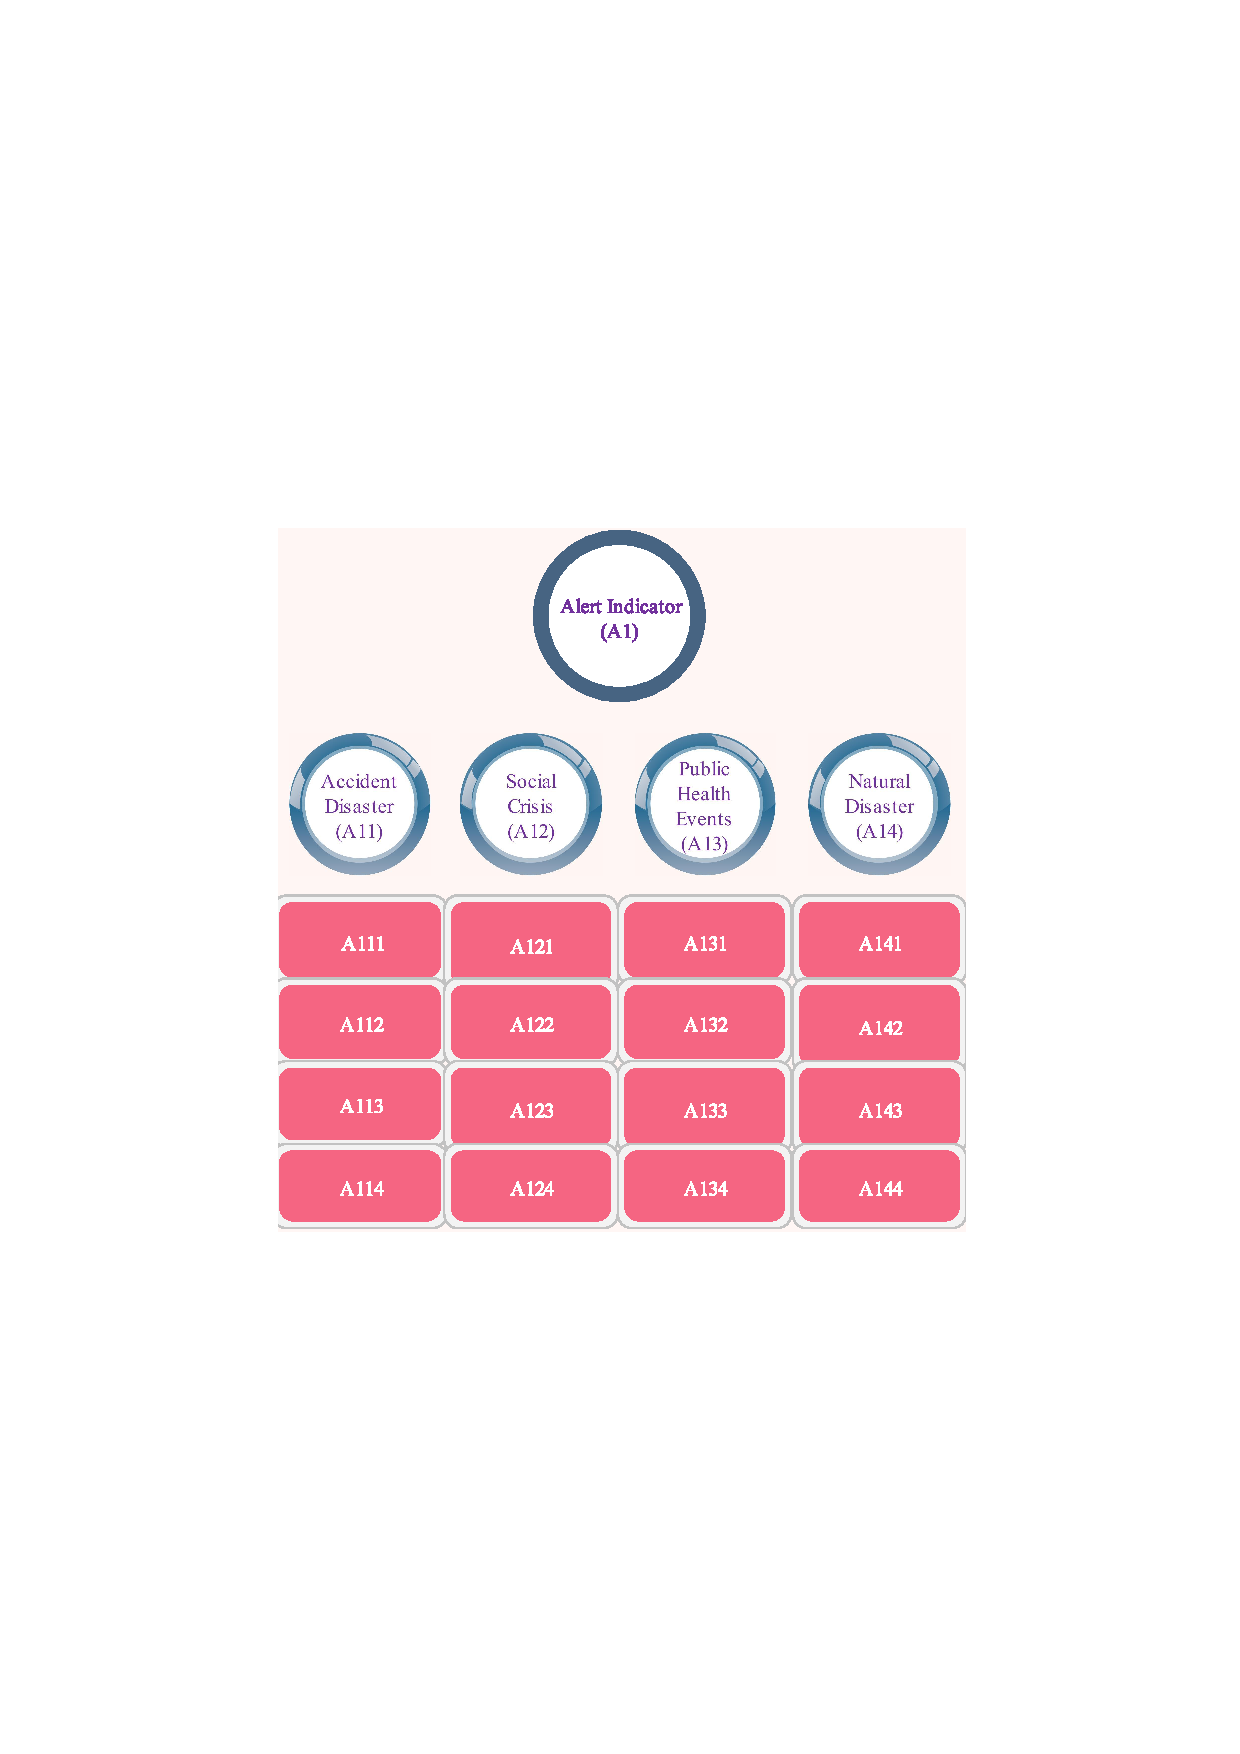
\includegraphics[width=\textwidth]{1}
\end{subfigure}
\begin{subfigure}[b]{.32\textwidth}
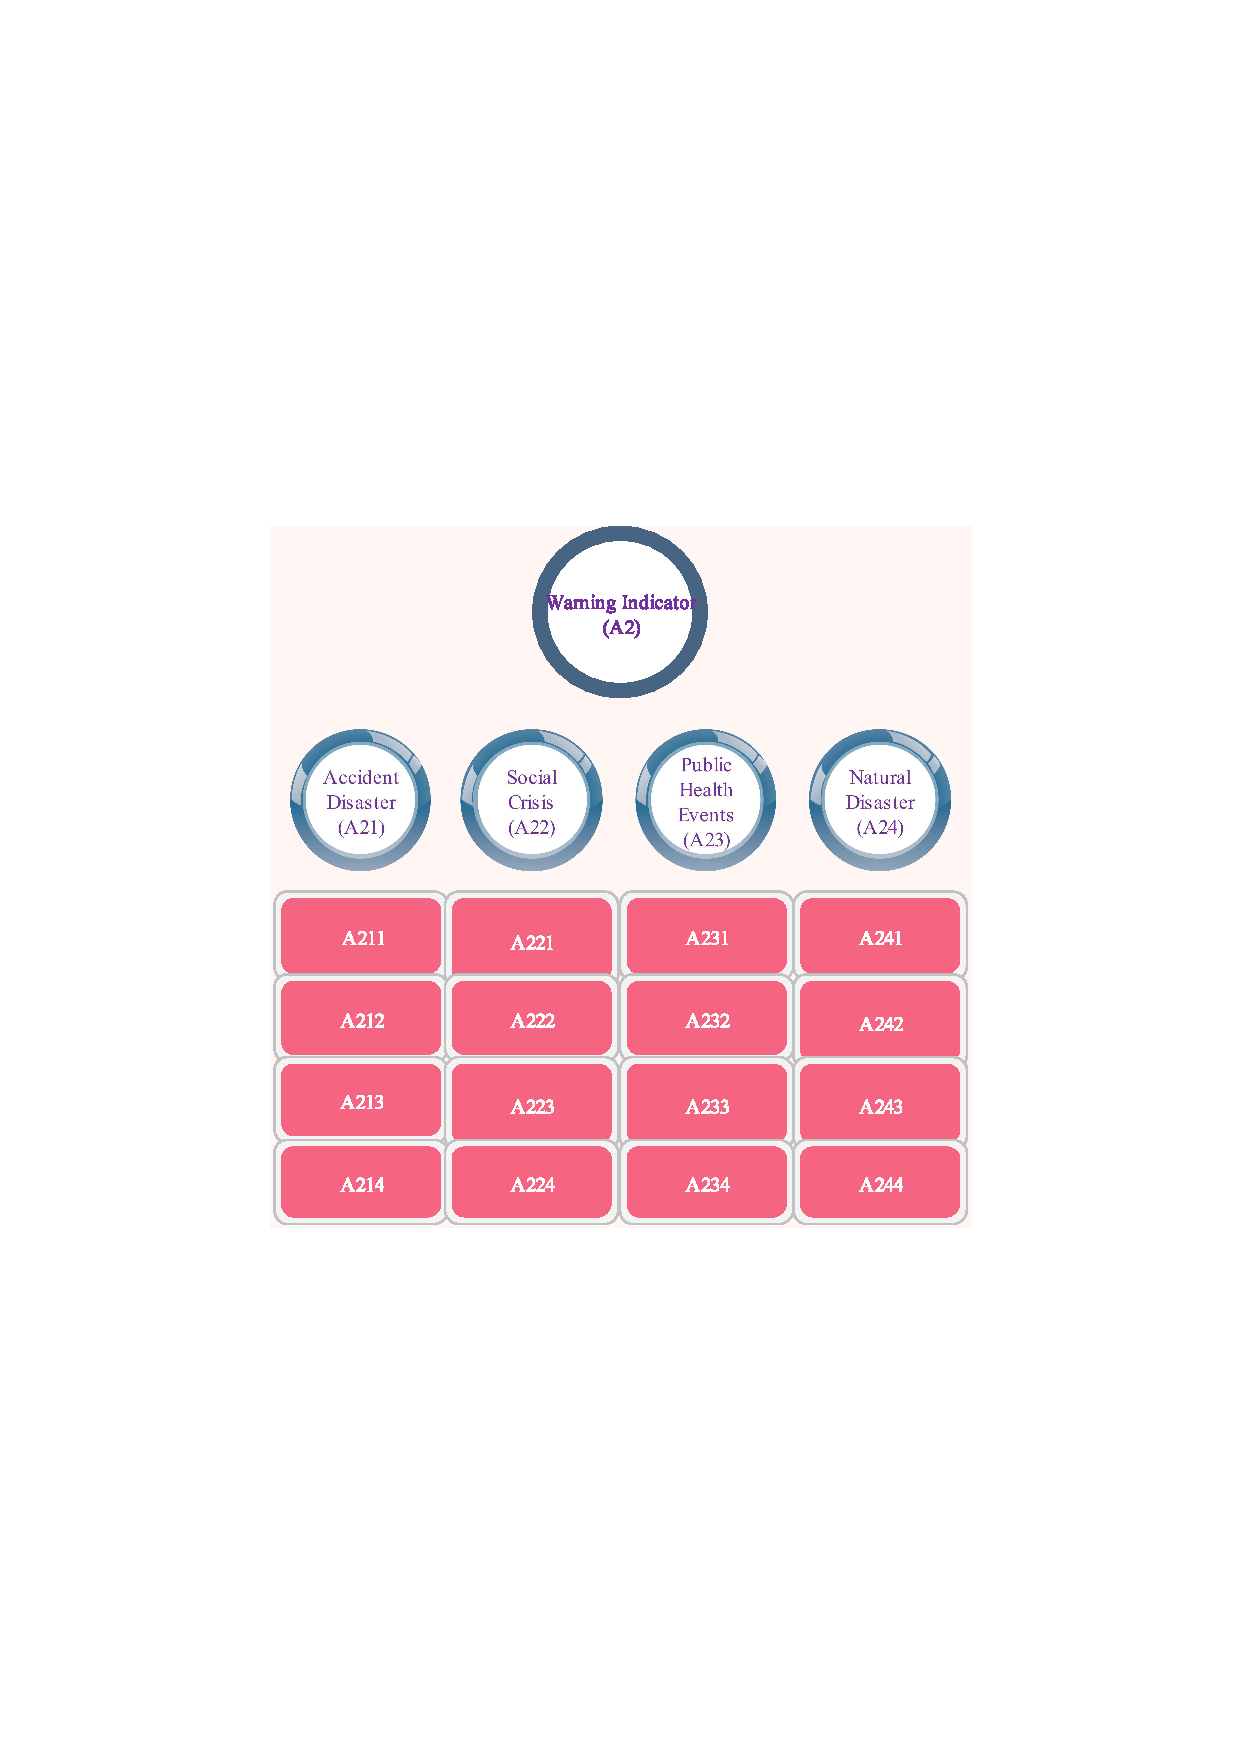
\includegraphics[width=\textwidth]{2}
\end{subfigure}
\begin{subfigure}[b]{.32\textwidth}
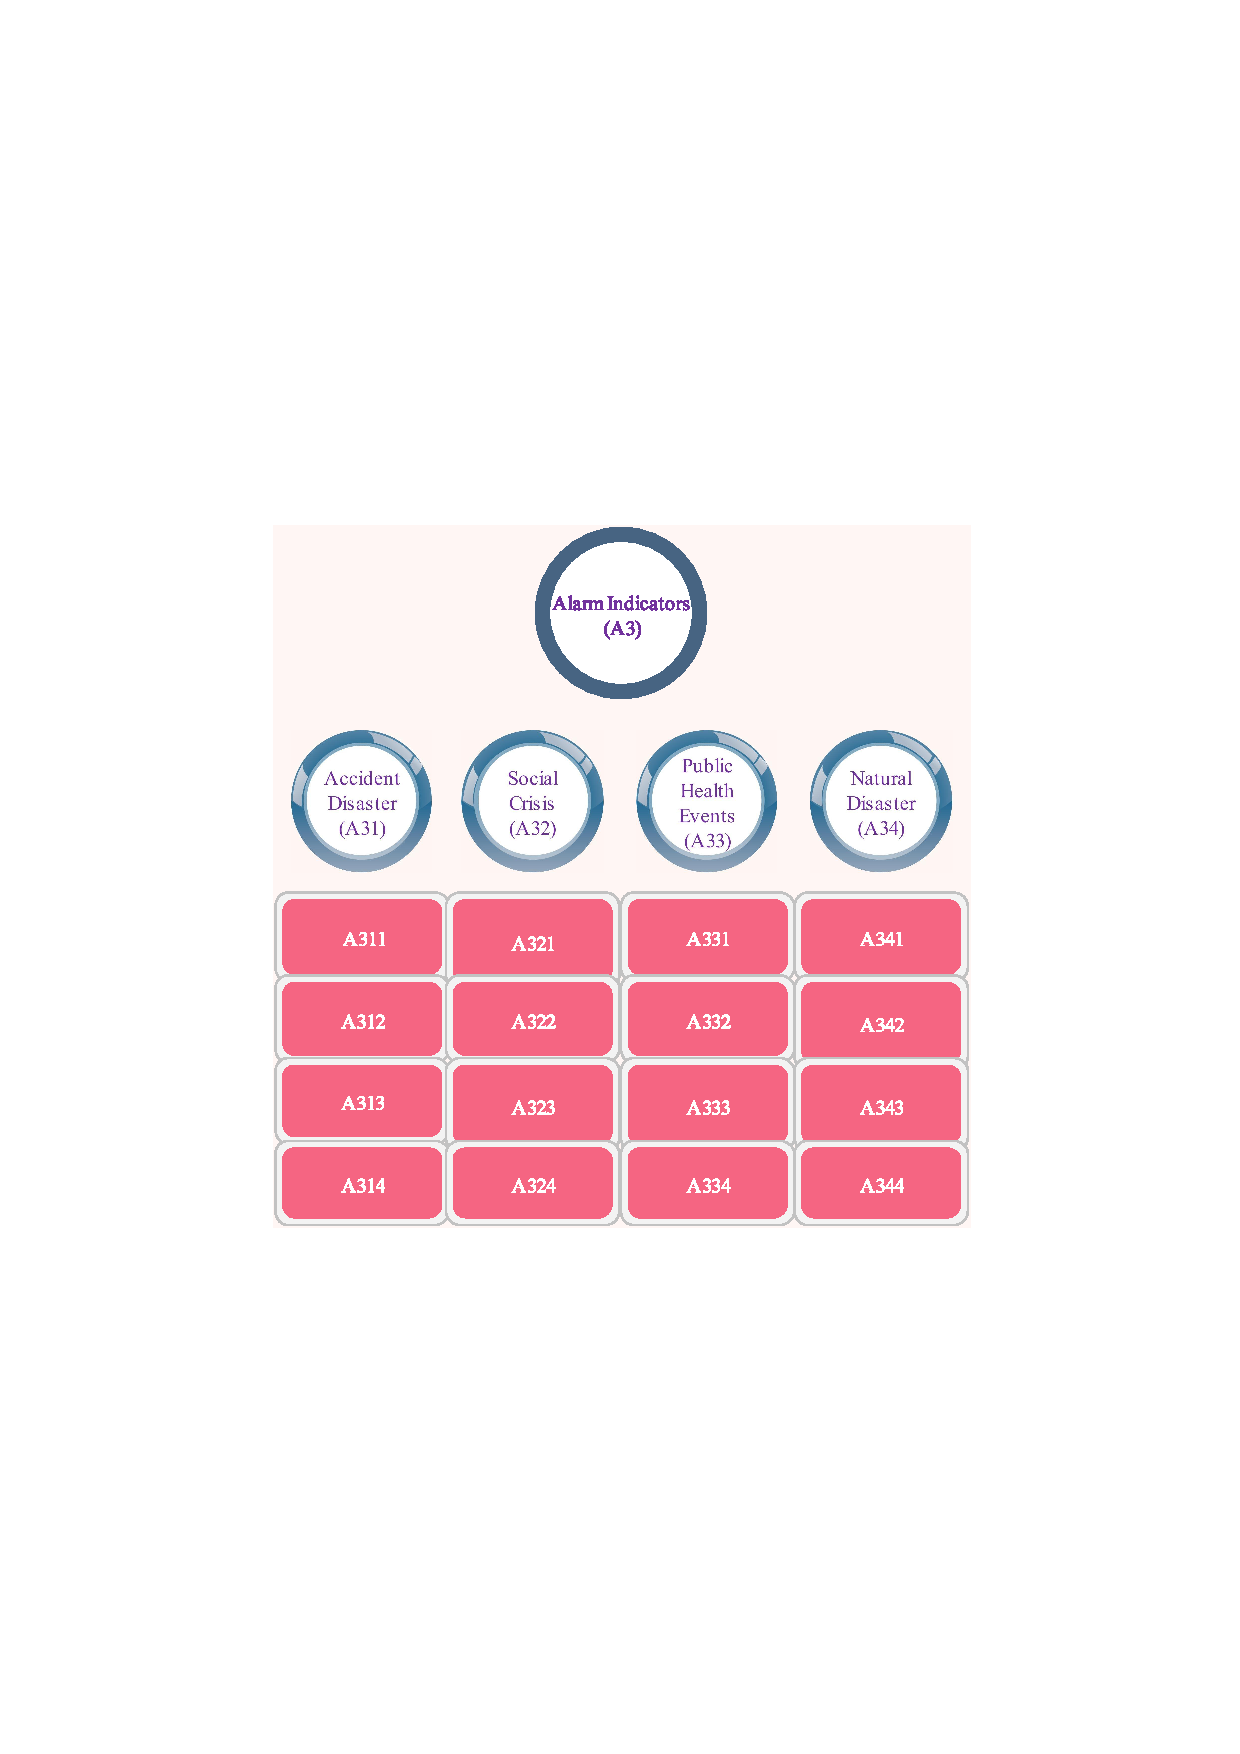
\includegraphics[width=\textwidth]{3}
\end{subfigure}
\caption{Selection of Indicators}\label{soi}
\end{figure}
\subsection{Establishment of Indicator System(Problem One)}
Here in order to more intuitively show the two matrices we have obtained, we will show the \textbf{Direct Influence Matrix} \bm{$W$}, \textbf{Comprehensive Influence Matrix} \bm{$T$} and the \textbf{The Reachability Matrix} \bm{$M$} in the form of Heatmap in the Figure \ref{heatmap}:
\begin{figure}[htbp]
\centering
\begin{subfigure}[b]{.32\textwidth}
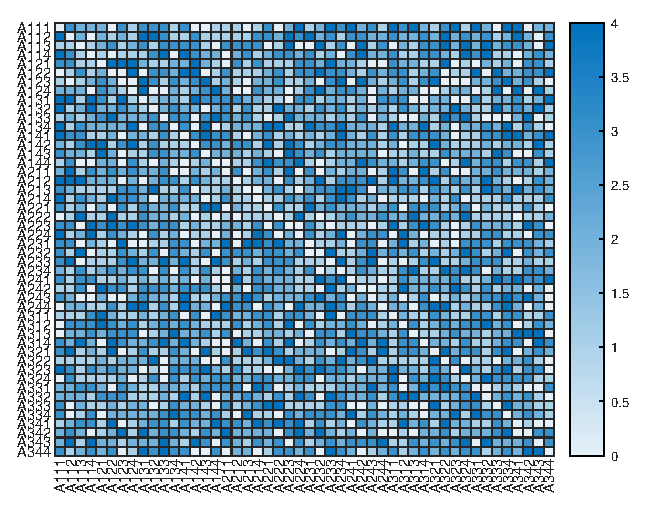
\includegraphics[width=\textwidth]{img/h2.eps}
\caption{Matrix $W$}
\end{subfigure}
\begin{subfigure}[b]{.32\textwidth}
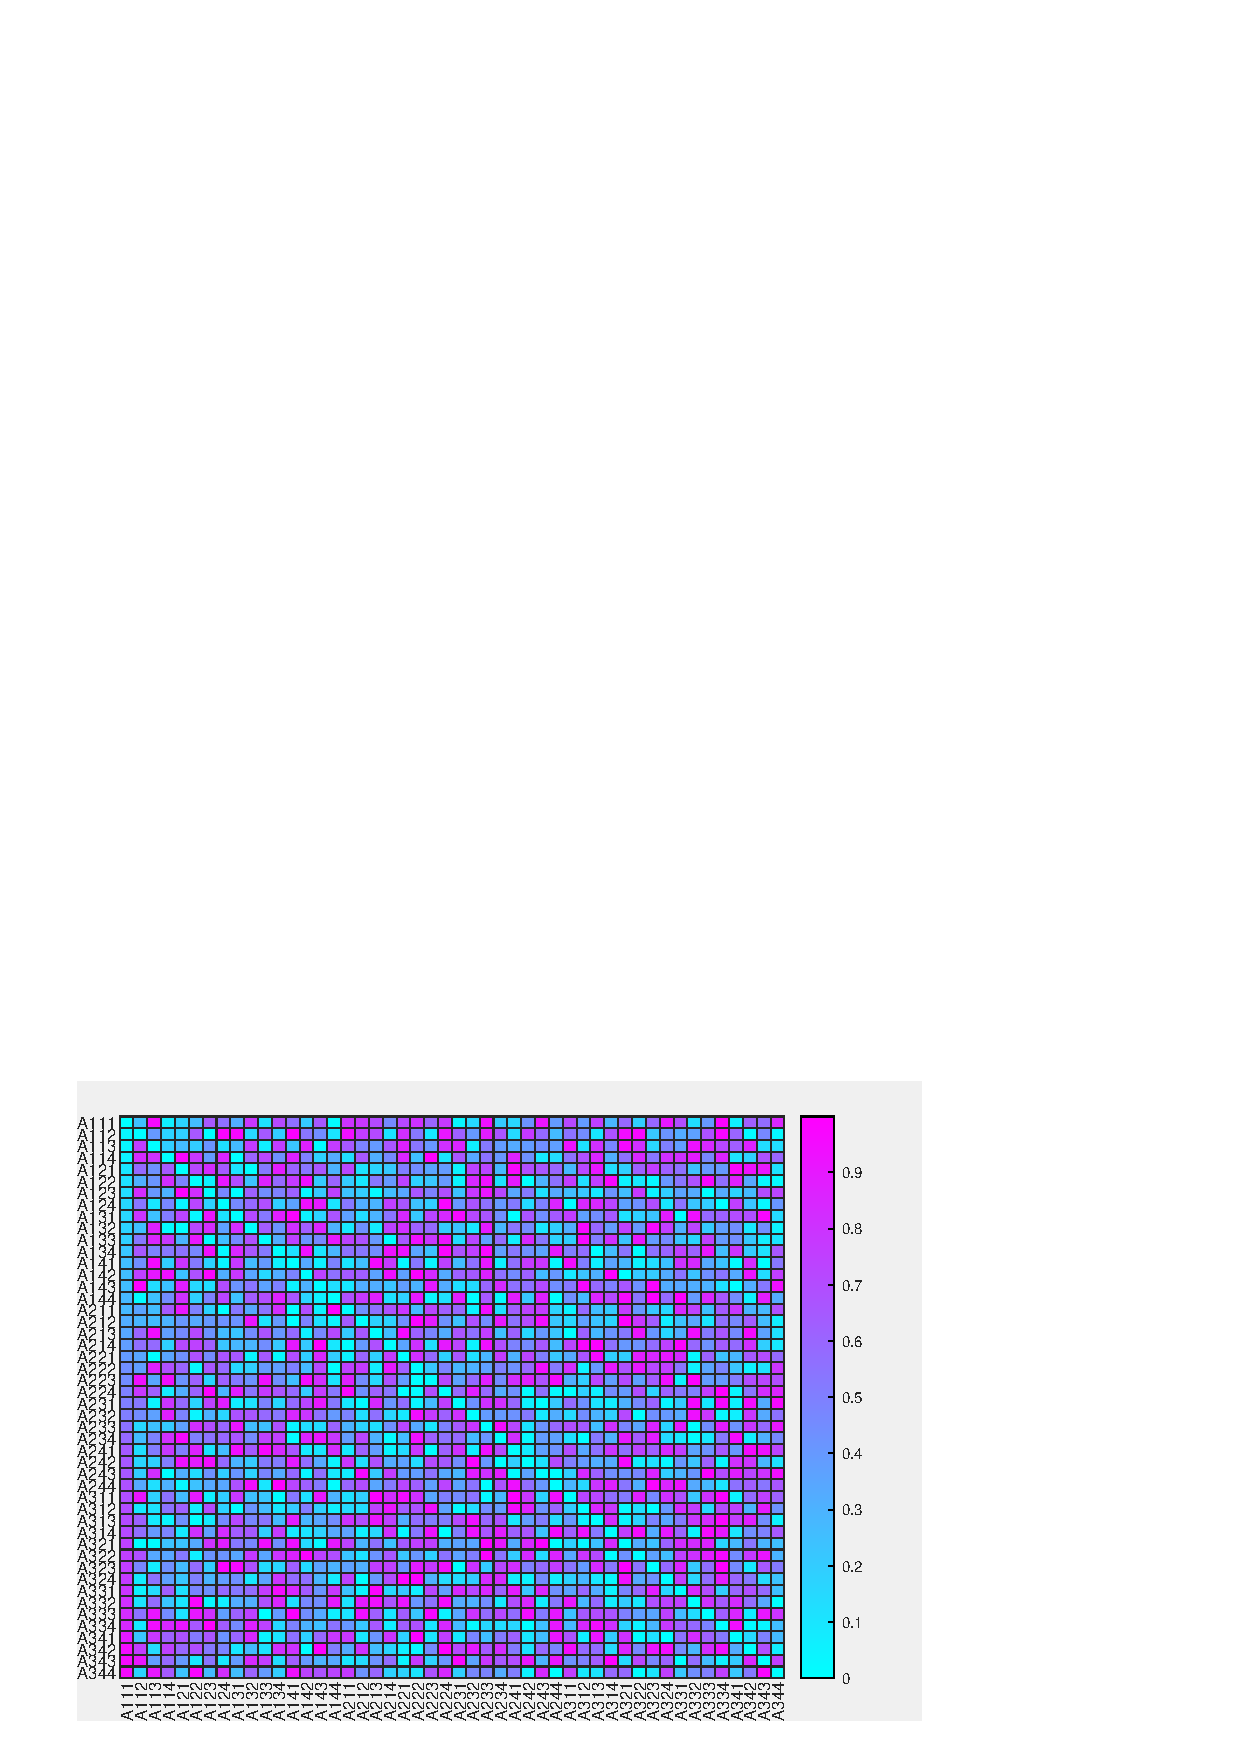
\includegraphics[width=\textwidth]{4}
\caption{Matrix $T$}
\end{subfigure}
\begin{subfigure}[b]{.32\textwidth}
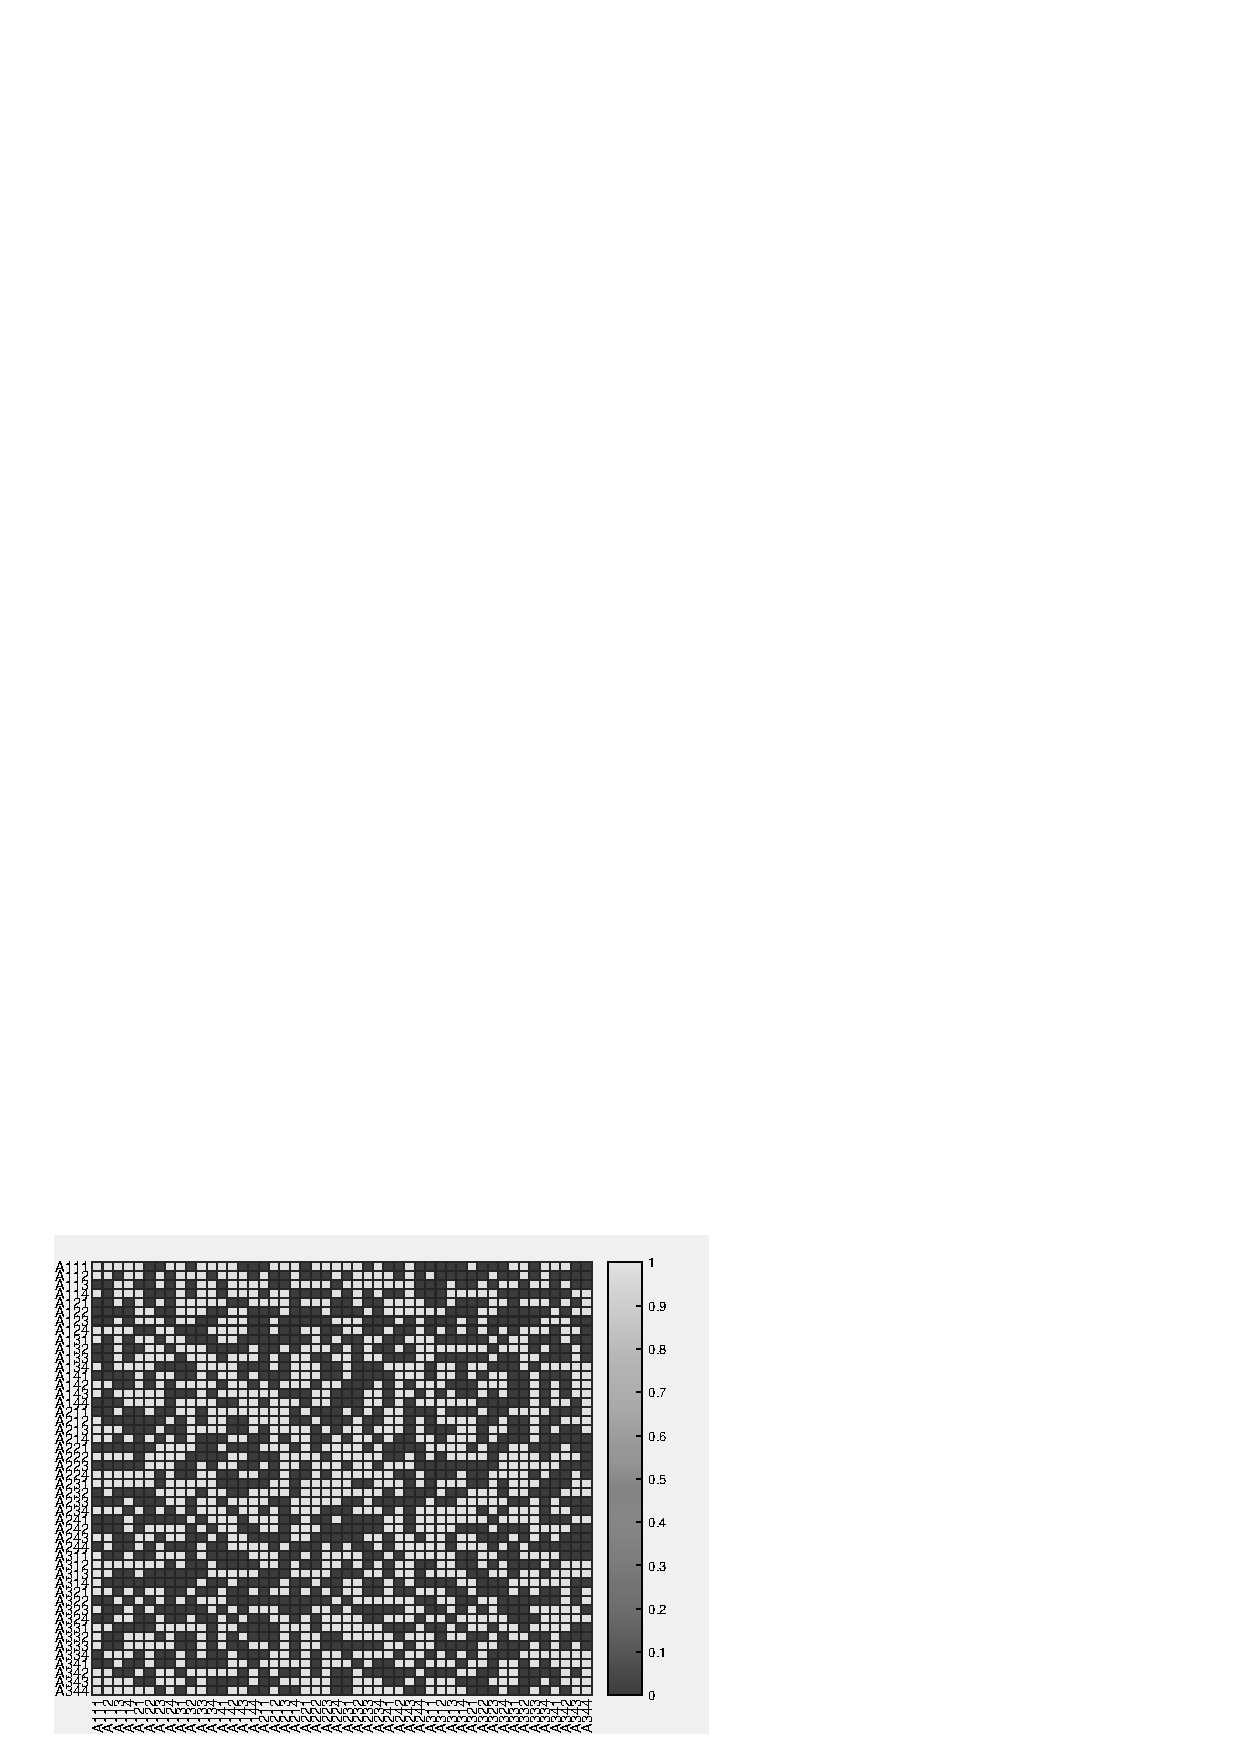
\includegraphics[width=\textwidth]{kdjz}
\caption{Matrix $M$}
\end{subfigure}
\caption{Heatmaps of Each Matrixes}
\label{heatmap}
\end{figure}

From the Heatmap above, we can easily see the relationship between the three indicators (1 in the matrix $M$ indicates that there is a relationship, 0 indicates that there is no relationship). According to our model, there is a positive correlation between the three indicators and the two indicators (we have carried out a positive treatment on the indicators).

At this time, the \textbf{Index System} we get is: with the \textbf{Alert Indicator($A_1$, Weight 0.390)}, \textbf{Warning Indicator($A_2$, Weight 0.319)}, and \textbf{Alarm Indicators($A_3$, Weight 0.291)} as the Level 1 indicators. Their secondary indicators are \textbf{Accident Disaster($A_{i1}$, Weight 0.123), Social Crisis($A_{i2}$, Weight 0.245), Public Health Events($A_{i3}$, Weight 0.491) }and \textbf{Natural Disaster($A_{i4}$, Weight 0.142)} respectively. Level 3 indicators and their weights are listed in the table.
\subsection{Solution For Problem Two}
We have established a social stability early warning model, which only needs to be scored according to the actual situation of each indicator, and the stability level can be obtained according to the final situation. But how to determine the score of each indicator we still need to discuss as follows:

Four aspects should be considered to determine the early warning level:
\subsubsection{Characteristic}
According to the predictability of its occurrence, it can be divided into sudden and recurrent. Due to their unpredictability, emergencies often have a strong impact on the people after they occur, thereby endangering social security and stability. Because regular events occur more frequently, the people have a certain ability to bear them, so when they occur, the intensity of the impact is less than that of sudden events. From the perspective of foreseeability, the warning level of sudden events should be higher than that of recurring events.

According to the relationship between its harm and residents, it can be divided into direct harm and indirect harm. As the direct hazard type is directly aimed at the personal safety of residents, it will cause great panic to residents once it occurs. The indirect hazard type will not directly threaten the personal safety of residents, so it is not easy to cause huge panic. As for the relationship between hazards and residents, the warning level of direct hazards should be higher than that of indirect hazards.

Considering the two kinds of nature of early warning events. From high to low, the early warning levels are \textbf{Sudden Direct Harm Type, Regular Direct Harm Type, Sudden Indirect Harm Type} and \textbf{Daily Indirect Harm Type}.
\subsubsection{Severity}
We have determined the severity of the incident in three respects: the level of threat to \textbf{The Lives of The Population, The Magnitude of The Economic Damage} and \textbf{The Potential of Further Harm}.
\subsubsection{Scope of Influence}
We believe that the influence scope can be measured from three aspects: \textbf{The Number of People Affected, The Impact of The Spatial Scope} and \textbf{The Impact of Psychological Degree}. The higher the number of residents involved in the incident, the higher the level of early warning; the greater the spatial scope of the incident, the higher the level of early warning; the stronger the psychological impact of the incident on the residents, the higher the level of early warning.
\subsubsection{Controllability}
We believe that people feel safe about situations they can control and fear situations they can't control, so event controllability affects the level of warning. The higher the degree of uncontrollability, the higher the warning level, and if it is completely out of control, it is extremely dangerous. Event controllability is measured from two aspects, namely, \textbf{The Understanding and Mastery of Relevant Factors} and \text{The Timely and Effective Degree of Measures}.

In the actual early warning, an event will have the above multiple attributes, so it is necessary to comprehensively analyze according to the specific situation and determine the early warning level of each indicator in the urban early warning indicator system.

When we determine the score of the indicator, we only need to bring in Equation \ref{eq} to get the warning level.



































\newpage







\clearpage
\subsubsection{Commetary on Model 2}
The instance of long and wide tables are shown in Table \ref{tb:longtable}.

% 长表格示例,更多用法请参考 longtable 宏包文档
% 以下环境及对应参数可实现表格内的自动换行与表格的自动断页
% 您也可以选择自行载入 tabularx 宏包,并通过 X 参数指定对应列自动换行
\begin{longtable}{ p{4em} p{14em} p{14em} }
\caption{Basic Information about Three Main Continents (scratched from Wikipedia)}
\label{tb:longtable}\\
\toprule
Continent & Description & Information \\
\midrule
Africa & Africa Continent is surrounded by the Mediterranean Sea to the
north, the Isthmus of Suez and the Red Sea to the northeast, the Indian
Ocean to the southeast and the Atlantic Ocean to the west. &
At about 30.3 million km$^2$ including adjacent islands, it covers 6\%
of Earth's total surface area and 20\% of its land area. With 1.3
billion people as of 2018, it accounts for about 16\% of the world's
human population. \\
\midrule
Asia & Asia is Earth's largest and most populous continent which
located primarily in the Eastern and Northern Hemispheres.
It shares the continental landmass of Eurasia with the continent
of Europe and the continental landmass of Afro-Eurasia with both
Europe and Africa. &
Asia covers an area of 44,579,000 square kilometres, about 30\%
of Earth's total land area and 8.7\% of the Earth's total surface
area. Its 4.5 billion people (as of June 2019) constitute roughly
60\% of the world's population. \\
\midrule
Europe & Europe is a continent located entirely in the Northern
Hemisphere and mostly in the Eastern Hemisphere. It comprises the
westernmost part of Eurasia and is bordered by the Arctic Ocean to
the north, the Atlantic Ocean to the west, the Mediterranean Sea to
the south, and Asia to the east. &
Europe covers about 10,180,000 km$^2$, or 2\% of the Earth's surface
(6.8\% of land area), making it the second smallest
continent. Europe had a total population of about 741 million (about
11\% of the world population) as of 2018. \\
\bottomrule
\end{longtable}
\section{Strengths and Weaknesses}
\subsection{Strengths}
\begin{itemize}
    \item First one...
    \item Second one ...
\end{itemize}

\subsection{Weaknesses}
\begin{itemize}
    \item Only one ...
 \end{itemize}










% 以下为信件/备忘录部分,不需要可自行去掉
% 如有需要可将整个 letter 环境移动到文章开头或中间
% 请在第二个花括号内填写标题,如「信件」(Letter)或「备忘录」(Memorandum)
\begin{letter}{Memorandum}
\begin{flushleft}  % 左对齐环境,无首行缩进
\textbf{To:} Heishan Yan\\
\textbf{From:} Team 1234567\\
\textbf{Date:} October 1st, 2019\\
\textbf{Subject:} A better choice than MS Word: \LaTeX
\end{flushleft}

In the memo, we want to introduce you an alternate typesetting program to the prevailing MS Word: \textbf{\LaTeX}. In fact, the history of \LaTeX\ is even longer than that of MS Word. In 1970s, the famous computer scientist Donald Knuth first came out with a typesetting program, which named \TeX\ \ldots

Firstly, \ldots

Secondly, \ldots

Lastly, \ldots

According to all those mentioned above, it is really worth to have a try on \LaTeX! 
\end{letter}


% 参考文献,此处以 MLA 引用格式为例
\begin{thebibliography}{99}
\bibitem{1} Einstein, A., Podolsky, B., \& Rosen, N. (1935). Can quantum-mechanical description of physical reality be considered complete?. \emph{Physical review}, 47(10), 777.
\bibitem{2} \emph{A simple, easy \LaTeX\ template for MCM/ICM: EasyMCM}. (2018). Retrieved December 1, 2019, from\url{https://www.cnblogs.com/xjtu-blacksmith/p/easymcm.html}
\end{thebibliography}


% 以下为附录内容
% 如您的论文中不需要附录,请自行删除
\begin{subappendices}  % 附录环境
\section{Appendix}
\begin{table}[!ht]\small
    \centering
    \caption{The Meaning and Weight of Each Indicator}
    \begin{tabular}{ccc}
        \hline
        Indicator & Indicator Layer &Weight\\ \hline
        A111 & Enterprise Loss Degree &0.014 \\ 
        A112 & Lack Of Investment In Urban Infrastructure &0.035 \\ 
        A113 & $\mathcal{D}$ Consistency Between The Urban Environment And Production &0.056 \\ 
        A114 & $\mathcal{D}$ Which Urban Policies Pay Attention To Production Safety &0.018 \\ 
        A121 & Crime Rate &0.030 \\ 
        A122 & Divorce Rate &0.099 \\ 
        A123 & Income Difference Degree Of Urban Residents &0.093 \\ 
        A124 & Urban Real Unemployment Rate &0.023 \\ 
        A131 & Development Degree Of Urban Health Sector&0.093  \\ 
        A132 & Concern About Urban Environmental Sanitation  &0.132\\ 
        A133 & Defense Against External Public Health Events &0.206 \\ 
        A134 & $\mathcal{D}$ Attention Paid By Urban Policies To Health Care &0.059 \\ 
        A141 & Extent Of Urban External Environment Damage&0.066  \\ 
        A142 & Climate Variability &0.022 \\ 
        A143 & Potential Threat To Urban Geological Structure&0.011  \\ 
        A144 &  Public Health&0.044 \\ 
        A211 & Frequency Of Production Accidents&0.048  \\ 
        A212 & Injury And Death Rate In Production Accidents&0.031  \\ 
        A213 & Damage Of Urban Infrastructure&0.010 \\ 
        A214 & Damage Degree Of Urban Infrastructure &0.034 \\ 
        A221 & Dissatisfaction With Social Order &0.049 \\ 
        A222 & Frequency Of Labor Disputes &0.057 \\ 
        A223 & Degree Of Pollution And Damage Accidents &0.080 \\ 
        A224 & Non-Institutionalized Group Development &0.059 \\ 
        A231 & Potential Occurrence And Activity Of Public Health Events &0.250 \\ 
        A232 & Active Degree Of Inducements For Public Health Events &0.184 \\ 
        A233 & Main Factors Of Natural Disasters &0.034\\ 
        A234 & Natural Disasters &0.023\\ 
        A241 & Instability Of Natural Disasters &0.055 \\ 
        A242 & Active Degree Of Main Factors Of Natural Disasters  &0.038\\ 
        A243 & Active Degree Of Natural Disaster Inducing Factors  &0.043\\ 
        A244 & Warfare Caused By Accidents And Disasters &0.007 \\ 
        A311 & Life Loss Caused By Accidents And Disasters &0.068 \\ 
        A312 & Economic Losses Caused By Accidents And Disasters  &0.055\\ 
        A313 & Group Crime &0.016 \\ 
        A314 & Group Fighting  &0.004\\ 
        A321 & Frequency And Scale Of Group Crime And Fighting&0.115  \\ 
        A322 & The Frequency And Scale Of Religious And Ethnic Conflicts &0.090 \\ 
        A323 & Active Degree Of Natural Disaster Inducing Factors  &0.008\\ 
        A324 & Warfare Caused By Public Health Events &0.009 \\ 
        A331 & Life Loss Caused By Public Health Events &0.217\\ 
        A332 & Economic Losses Caused By Public Health Events &0.159 \\ 
        A333 & Psychological Problems Caused By Public Health Events &0.115 \\ 
        A334 & Life Loss &0.003 \\ 
        A341 & Degree Of Life Loss &0.046\\ 
        A342 & Property Damage Degree&0.029  \\ 
        A343 & Degree Of Direct Production Loss&0.051  \\ 
        A344 & Indirect Loss Degree Of Natural Disasters&0.016  \\ \hline
    \end{tabular}
\end{table}

\end{subappendices}  % 附录内容结束



















































\end{document}  % 结束
